% Options for packages loaded elsewhere
\PassOptionsToPackage{unicode}{hyperref}
\PassOptionsToPackage{hyphens}{url}
%
\documentclass[openany,twoside]{book}
\usepackage{lmodern}
\usepackage{amssymb,amsmath}
\usepackage{geometry}
\geometry{margin=.9in}
\usepackage{ifxetex,ifluatex}
\ifnum 0\ifxetex 1\fi\ifluatex 1\fi=0 % if pdftex
  \usepackage[T1]{fontenc}
  \usepackage[utf8]{inputenc}
  \usepackage{textcomp} % provide euro and other symbols
\else % if luatex or xetex
  \usepackage{unicode-math}
  \defaultfontfeatures{Scale=MatchLowercase}
  \defaultfontfeatures[\rmfamily]{Ligatures=TeX,Scale=1}
\fi
% Use upquote if available, for straight quotes in verbatim environments
\IfFileExists{upquote.sty}{\usepackage{upquote}}{}
\IfFileExists{microtype.sty}{% use microtype if available
  \usepackage[]{microtype}
  \UseMicrotypeSet[protrusion]{basicmath} % disable protrusion for tt fonts
}{}
\makeatletter
\@ifundefined{KOMAClassName}{% if non-KOMA class
  \IfFileExists{parskip.sty}{%
    \usepackage{parskip}
  }{% else
    \setlength{\parindent}{0pt}
    \setlength{\parskip}{6pt plus 2pt minus 1pt}}
}{% if KOMA class
  \KOMAoptions{parskip=half}}
\makeatother
\usepackage{xcolor}
\IfFileExists{xurl.sty}{\usepackage{xurl}}{} % add URL line breaks if available
\IfFileExists{bookmark.sty}{\usepackage{bookmark}}{\usepackage{hyperref}}
\hypersetup{
  pdftitle={Binary classification as a phase separation process - a short tutorial},
  hidelinks,
  colorlinks = true,
            linkcolor = brown,
            urlcolor  = blue,
            citecolor = blue,
  pdfcreator={LaTeX via pandoc}}
\urlstyle{same} % disable monospaced font for URLs
\usepackage{color}
\usepackage{fancyvrb}
\newcommand{\VerbBar}{|}
\newcommand{\VERB}{\Verb[commandchars=\\\{\}]}
\DefineVerbatimEnvironment{Highlighting}{Verbatim}{commandchars=\\\{\}}
% Add ',fontsize=\small' for more characters per line
\usepackage{framed}
\definecolor{shadecolor}{RGB}{248,248,248}
\newenvironment{Shaded}{\begin{snugshade}}{\end{snugshade}}
\newcommand{\AlertTok}[1]{\textcolor[rgb]{0.94,0.16,0.16}{#1}}
\newcommand{\AnnotationTok}[1]{\textcolor[rgb]{0.56,0.35,0.01}{\textbf{\textit{#1}}}}
\newcommand{\AttributeTok}[1]{\textcolor[rgb]{0.77,0.63,0.00}{#1}}
\newcommand{\BaseNTok}[1]{\textcolor[rgb]{0.00,0.00,0.81}{#1}}
\newcommand{\BuiltInTok}[1]{#1}
\newcommand{\CharTok}[1]{\textcolor[rgb]{0.31,0.60,0.02}{#1}}
\newcommand{\CommentTok}[1]{\textcolor[rgb]{0.56,0.35,0.01}{\textit{#1}}}
\newcommand{\CommentVarTok}[1]{\textcolor[rgb]{0.56,0.35,0.01}{\textbf{\textit{#1}}}}
\newcommand{\ConstantTok}[1]{\textcolor[rgb]{0.00,0.00,0.00}{#1}}
\newcommand{\ControlFlowTok}[1]{\textcolor[rgb]{0.13,0.29,0.53}{\textbf{#1}}}
\newcommand{\DataTypeTok}[1]{\textcolor[rgb]{0.13,0.29,0.53}{#1}}
\newcommand{\DecValTok}[1]{\textcolor[rgb]{0.00,0.00,0.81}{#1}}
\newcommand{\DocumentationTok}[1]{\textcolor[rgb]{0.56,0.35,0.01}{\textbf{\textit{#1}}}}
\newcommand{\ErrorTok}[1]{\textcolor[rgb]{0.64,0.00,0.00}{\textbf{#1}}}
\newcommand{\ExtensionTok}[1]{#1}
\newcommand{\FloatTok}[1]{\textcolor[rgb]{0.00,0.00,0.81}{#1}}
\newcommand{\FunctionTok}[1]{\textcolor[rgb]{0.00,0.00,0.00}{#1}}
\newcommand{\ImportTok}[1]{#1}
\newcommand{\InformationTok}[1]{\textcolor[rgb]{0.56,0.35,0.01}{\textbf{\textit{#1}}}}
\newcommand{\KeywordTok}[1]{\textcolor[rgb]{0.13,0.29,0.53}{\textbf{#1}}}
\newcommand{\NormalTok}[1]{#1}
\newcommand{\OperatorTok}[1]{\textcolor[rgb]{0.81,0.36,0.00}{\textbf{#1}}}
\newcommand{\OtherTok}[1]{\textcolor[rgb]{0.56,0.35,0.01}{#1}}
\newcommand{\PreprocessorTok}[1]{\textcolor[rgb]{0.56,0.35,0.01}{\textit{#1}}}
\newcommand{\RegionMarkerTok}[1]{#1}
\newcommand{\SpecialCharTok}[1]{\textcolor[rgb]{0.00,0.00,0.00}{#1}}
\newcommand{\SpecialStringTok}[1]{\textcolor[rgb]{0.31,0.60,0.02}{#1}}
\newcommand{\StringTok}[1]{\textcolor[rgb]{0.31,0.60,0.02}{#1}}
\newcommand{\VariableTok}[1]{\textcolor[rgb]{0.00,0.00,0.00}{#1}}
\newcommand{\VerbatimStringTok}[1]{\textcolor[rgb]{0.31,0.60,0.02}{#1}}
\newcommand{\WarningTok}[1]{\textcolor[rgb]{0.56,0.35,0.01}{\textbf{\textit{#1}}}}
\usepackage{longtable,booktabs}
% Correct order of tables after \paragraph or \subparagraph
\usepackage{etoolbox}
\makeatletter
\patchcmd\longtable{\par}{\if@noskipsec\mbox{}\fi\par}{}{}
\makeatother
% Allow footnotes in longtable head/foot
\IfFileExists{footnotehyper.sty}{\usepackage{footnotehyper}}{\usepackage{footnote}}
\makesavenoteenv{longtable}
\usepackage{graphicx,grffile}
\makeatletter
\def\maxwidth{\ifdim\Gin@nat@width>\linewidth\linewidth\else\Gin@nat@width\fi}
\def\maxheight{\ifdim\Gin@nat@height>\textheight\textheight\else\Gin@nat@height\fi}
\makeatother
% Scale images if necessary, so that they will not overflow the page
% margins by default, and it is still possible to overwrite the defaults
% using explicit options in \includegraphics[width, height, ...]{}
\setkeys{Gin}{width=\maxwidth,height=\maxheight,keepaspectratio}
% Set default figure placement to htbp
\makeatletter
\def\fps@figure{htbp}
\makeatother
\setlength{\emergencystretch}{3em} % prevent overfull lines
\providecommand{\tightlist}{%
  \setlength{\itemsep}{0pt}\setlength{\parskip}{0pt}}
\setcounter{secnumdepth}{5}
\usepackage{booktabs}
\usepackage[]{natbib}
\bibliographystyle{apalike}
%%%%%%%%%%%%%%%%%%%%%%%%%%%%%%%%%%%%%

\usepackage{fancyhdr}
\usepackage{lipsum}% just to generate text for the example

\newcommand\shorttitle{Binary classification as a phase separation process - a short tutorial }
\newcommand\authors{Rafael Monteiro}

\fancyhf{}
\renewcommand\headrulewidth{0pt}
\fancyhead[CE]{\small\scshape\shorttitle}
\fancyhead[CO]{\small\scshape\authors}
\pagestyle{fancy}




\title{Binary classification as a phase separation process - a short tutorial to the implemented model}
\author{Rafael Monteiro}
\date{2020-09-17}

\begin{document}
\maketitle

{
\setcounter{tocdepth}{1}
\tableofcontents
}
\hypertarget{intro}{%
\chapter{Introduction}\label{intro}}

This is a short companion tutorial to the github \citep{Bin_phase_github}. We give here a glimpse of the Phase Separation Binary Classifier (in short, PSBC), proposed in the article \textbf{Binary Classification as a Phase Separation Process}, by \href{https://sites.google.com/view/rafaelmonteiro-math/home}{Rafael Monteiro}; a \href{https://arxiv.org/abs/2009.02467}{preprint} is available on arXiv.

An implementation of the model can be found in the module \textbf{binary\_phase\_separation.py}. Part of this tutorial can also be found in \href{https://github.com/rafael-a-monteiro-math/Binary_classification_phase_separation/blob/master/README.pdf}{README.pdf}.

\textbf{\ldots but, before we start\ldots{}}

\begin{itemize}
\item
  The main module for this project is \textbf{binary\_phase\_separation.py}, that you will find in this Github page \citep{Bin_phase_github}.
\item
  If you are looking for the dataset and trained models, see the \citep{Bin_phase_data} at Zenodo.
\item
  If you want to reproduce this notebook you should download the file \href{https://zenodo.org/record/4005131/files/PSBC_Examples.tar.gz?download=1}{PSBC\_Examples.tar.gz} in the aforementioned data repository, and also the tarball \href{https://github.com/rafael-a-monteiro-math/Binary_classification_phase_separation/blob/master/PSBC_Notebooks.tar.gz}{jupyter-notebooks} in \citep{Bin_phase_github}.\footnote{This tarball contains all the 3 notebooks, and also the two modules used.}
\item
  To download data, I highly recommend the use of the script \href{https://github.com/rafael-a-monteiro-math/Binary_classification_phase_separation/blob/master/download_PSBC.sh}{download\_PSBC.sh}, for a few reasons: (i) it downloads the data in a safe way (using \href{https://www.gnu.org/software/wget/}{wget}); (ii) it automatically checks the MD5 of each file. We would like to highlight that you can also use the same script to download only the \href{https://zenodo.org/record/4005131/files/PSBC_Examples.tar.gz?download=1}{trained examples} and only the \href{https://github.com/rafael-a-monteiro-math/Binary_classification_phase_separation/blob/master/PSBC_Notebooks.tar.gz}{jupyter-notebooks} for this project. In order to use it, please read first \href{https://github.com/rafael-a-monteiro-math/Binary_classification_phase_separation/blob/master/README.pdf}{this README.pdf} guide for further explanation.
\item
  This website is based on \href{Notebook_PSBC_example.ipynb}{this jupyter-notebook}. The full code to the pictures seen here are posted there. For that reason, I shall refrain from posting the whole oputput of some cases, marking then with a symbol \(>>>\).
\item
  We will summarize some of the outputs, adding a ``\ldots{}'' to them. If you would like to see the whole output, please see \href{https://github.com/rafael-a-monteiro-math/Binary_classification_phase_separation/blob/master/Notebook_PSBC_examples.ipynb}{Notebook\_PSBC\_example.ipynb}.
\end{itemize}

As we said, this discussion is short but we want to offer a bit more than just a manual, so we will point out references along the way.

\hypertarget{a_few_examples}{%
\chapter{Nonlinear diffusion equations: a numerical example}\label{a_few_examples}}

To begin with, I will introduce the model, giving some examples of its use. Let's first import some libraries

\begin{Shaded}
\begin{Highlighting}[]
\ImportTok{from}\NormalTok{ sklearn.model_selection }\ImportTok{import}\NormalTok{ train_test_split, StratifiedKFold}
\ImportTok{from}\NormalTok{ sklearn.preprocessing }\ImportTok{import}\NormalTok{ MinMaxScaler}
\ImportTok{import}\NormalTok{ matplotlib.gridspec }\ImportTok{as}\NormalTok{ gridspec}
\NormalTok{...}
\end{Highlighting}
\end{Shaded}

As discussed in Section 1.1 in the paper, the nonlinear diffusion processes are in the backdrop of this model. The heart of the model is the Allen-Cahn equation \citep{Fife},\citep{Ar_Wein},\citep{allen1979microscopic}, a well-known equation in the field of pattern formation. Just to show how part of the PSBC's implementation can be used to evolve an initial boundary value problem with Neumann boundary conditions: we shall take

\begin{equation}
u_0(x) = \frac{1- \sin(\pi(2x - 1))}{2}\label{eq:1}
\end{equation}

as an initial condition to the Allen-Cahn equation

\begin{equation}
\partial_tu(x, t) = \varepsilon^2 \partial_x^2u(x, t) + u(x, t)(1 -  u(x, t))(u(x, t) - \alpha(x)).\label{eq:2}
\end{equation}

The parameter \(\alpha(\cdot)\) embodies medium heterogeneity. In the case shown here, we choose \(\alpha(x) = -2\), when \(x <0.5\), and \(\alpha(x)\) = 2, when \(x \geq 0.5\).

Parameters to the model are assigned below:

\begin{Shaded}
\begin{Highlighting}[]
\NormalTok{N }\OperatorTok{=} \DecValTok{20}
\NormalTok{x }\OperatorTok{=}\NormalTok{ np.linspace(}\DecValTok{0}\NormalTok{, }\DecValTok{1}\NormalTok{, N, endpoint }\OperatorTok{=} \VariableTok{True}\NormalTok{)}
\NormalTok{V_0 }\OperatorTok{=} \DecValTok{1}\OperatorTok{/}\DecValTok{2} \OperatorTok{-} \DecValTok{1}\OperatorTok{/}\DecValTok{2} \OperatorTok{*}\NormalTok{ np.reshape(np.sin(np.pi }\OperatorTok{*}\NormalTok{ (}\DecValTok{2} \OperatorTok{*}\NormalTok{ x }\OperatorTok{-} \DecValTok{1}\NormalTok{)) , (}\OperatorTok{-}\DecValTok{1}\NormalTok{,}\DecValTok{1}\NormalTok{))}
\NormalTok{prop }\OperatorTok{=}\NormalTok{ Propagate()}
\NormalTok{dt, eps, Nx, Nt }\OperatorTok{=} \FloatTok{0.1}\NormalTok{, }\FloatTok{.3}\NormalTok{,  N, }\DecValTok{400}
\NormalTok{dx, ptt_cardnlty, weigths_k_sharing }\OperatorTok{=}\NormalTok{ x[}\DecValTok{1}\NormalTok{]}\OperatorTok{-}\NormalTok{x[}\DecValTok{0}\NormalTok{], Nx, Nt}
\end{Highlighting}
\end{Shaded}

Then we initialize parameters

\begin{Shaded}
\begin{Highlighting}[]
\NormalTok{init }\OperatorTok{=}\NormalTok{ Initialize_parameters()}
\NormalTok{param }\OperatorTok{=}\NormalTok{ init.dictionary(N, eps, dt, dx, Nt, ptt_cardnlty, weigths_k_sharing)}
\end{Highlighting}
\end{Shaded}

If you read the paper you remember that trainable weights are the coefficients of this PDE. Since the model randomly initialize these coefficients, we will have to readjust them to the value we want. That's what we do in the next part of the code.

\begin{Shaded}
\begin{Highlighting}[]
\ControlFlowTok{for}\NormalTok{ i }\KeywordTok{in} \BuiltInTok{range}\NormalTok{(param[}\StringTok{"Nt"}\NormalTok{]):}
\NormalTok{	param[}\StringTok{"alpha_x_t"}\NormalTok{][:,i] }\OperatorTok{=} \DecValTok{-2} \OperatorTok{*}\NormalTok{ (x }\OperatorTok{<} \FloatTok{.5}\NormalTok{) }\OperatorTok{+} \DecValTok{2} \OperatorTok{*}\NormalTok{ (x }\OperatorTok{>=} \FloatTok{.5}\NormalTok{)}
\end{Highlighting}
\end{Shaded}

which we now run, using the numerical scheme (1.7a) in the paper. Recall that this step is the same as doing a forward propagation in a feed forward network: that's the reason why you see the method ``prop.forward'' in the code below.

\begin{Shaded}
\begin{Highlighting}[]
\NormalTok{flow, waterfall, time }\OperatorTok{=}\NormalTok{ prop.forward(V_0, param, waterfall_save }\OperatorTok{=} \VariableTok{True}\NormalTok{ , Flow_save }\OperatorTok{=} \VariableTok{True}\NormalTok{)}
\NormalTok{time }\OperatorTok{=}\NormalTok{ np.arange(Nt }\OperatorTok{+} \DecValTok{1}\NormalTok{)}
\NormalTok{X, Y }\OperatorTok{=}\NormalTok{ np.meshgrid(x, time)}
\NormalTok{flow }\OperatorTok{=}\NormalTok{ np.squeeze(flow, axis }\OperatorTok{=} \DecValTok{1}\NormalTok{)}
\end{Highlighting}
\end{Shaded}

When we plot the evolution of \(u_0(\cdot)\) through the Allen-Cahn equation as a surface, we get the plot below (code in \href{https://github.com/rafael-a-monteiro-math/Binary_classification_phase_separation/blob/master/Notebook_PSBC_examples.ipynb}{Notebook\_examples.ipynb}).

\begin{figure}
\centering
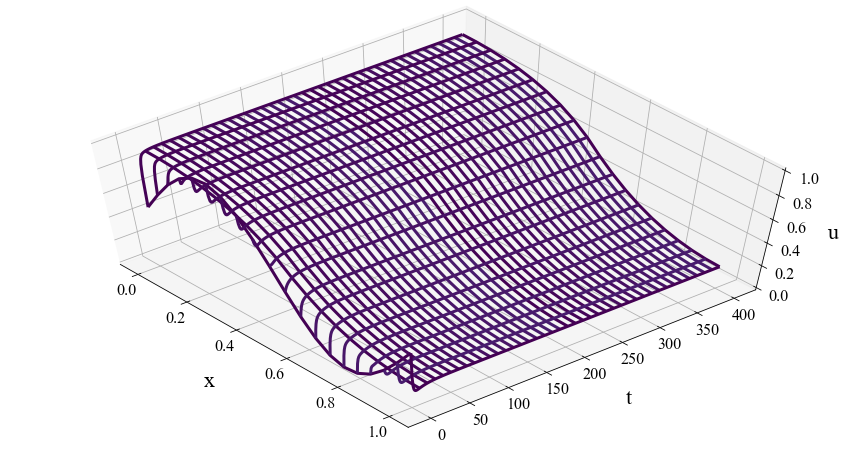
\includegraphics{figures/output_11_0.png}
\caption{The initial condition \(u_0(\cdot)\) shown in Equation \eqref{eq:1}, as it evolves according to the Allen-Cahn equation \eqref{eq:2}.}
\end{figure}

One of the first motivations to this project can be found in the interesting paper \citep{Ang_Mal}, where they have shown that several nontrivial layered patterns\^{}\{Stationary solutions to equation \eqref{eq:2} that, roughly speaking, gets ``concentrated'' around values 0 and 1, displaying layers in between these values.\} can be found if \(\alpha(\cdot)\) is non-homogeneous in space. There is an extensive discussion about why this is interesting, and we refer the reader to Section 1.1 in the paper.

\begin{quote}
\textbf{Remark:} You can read more about pattern formation in the book \citep{Nishiura} (Chapter 4.2 deals with the Allen-Cahn model), and also in the very nice article Arnd Scheel wrote to the Princeton Companion to Applied Mathematics, Section IV. 27 \citep{Arnd_companion}.
\end{quote}

\hypertarget{propagation-with-randomly-generated-coefficients}{%
\section{Propagation with randomly generated coefficients}\label{propagation-with-randomly-generated-coefficients}}

Next, we would like to evolve and plot the evolution of several different initial conditions in the interval {[}0,1{]} (code in \href{https://github.com/rafael-a-monteiro-math/Binary_classification_phase_separation/blob/master/Notebook_PSBC_examples.ipynb}{Notebook\_examples.ipynb}). The model that we use is, initially, a discretization of \eqref{eq:2}, with \(\varepsilon = 0\), which then becomes an ODE:

\begin{equation}
U^{[n+1]} = U^{[n]} + \Delta_t^{u}f(U^{[n]},\alpha^{[n]}),\label{eq:3}
\end{equation}

where \(f(U^{[n]},\alpha^{[n]}):= U^{[n]}(1 - U^{[n]})(U^{[n]} - \alpha^{[n]} )\).

It is good to have in mind that the coefficients in the above ODE will play the role of trainable weights in Machine Learning: we will ``adjust'' the coefficients in \(\alpha(\cdot)\) in order to achieve a certain final, target end state.

As mentioned earlier, there is a clear correspondence between the initial value (ODE/PDE) problem and forward propagation and, consequently, the stability of \eqref{eq:3} has to be considered. The discretization it presents is known as (explicit) Euler method, which is known to be (linearly) unstable in many cases. A good part of the paper was devoted to showing that there is some kind of \emph{nonlinear stabilization} mechanism that prevents solutions from blowing up, a condition referred to as \emph{Invariant Region Enforcing Condition}, which establishes a critical threshold for the size of \(\Delta_t^u\), beyond which solutions can blow up. This is discussed at lenght in the \href{https://arxiv.org/abs/2009.02467}{paper}.

To get this critical value for \(\Delta_t^u\) it is necessary to quantify

\begin{equation}
\max_{1\leq k \leq \mathrm{N_t}}\max\{1,\vert \alpha^{[k]}\vert\} <+\infty,\label{eq:boundedness}
\end{equation}

based on which we adjust the parameter \(\Delta_t^u\) accordingly, in a nontrivial way.\^{}\{Because, of course, \(\Delta_t^u =0\) also does the job, but does not deliver what we want.\} In result, the evolution of \(U^{[\cdot]}\) does not end up in a floating point overflow (in other words, a blow up in \(\ell^{\infty}\) norm).

We set up a little experiment, where in some we obey the \emph{Invariant Region Enforcing Condition}, and in some we don't. We take several initial condition on the interval \([0,1]\) and evolving them according to \eqref{eq:3}. Parameters are as follows:

\begin{Shaded}
\begin{Highlighting}[]
\NormalTok{N }\OperatorTok{=} \DecValTok{1}
\NormalTok{init }\OperatorTok{=}\NormalTok{ Initialize_parameters()}
\NormalTok{prop }\OperatorTok{=}\NormalTok{ Propagate()}
\NormalTok{dt_vec }\OperatorTok{=}\NormalTok{ np.array([.}\DecValTok{1}\NormalTok{,.}\DecValTok{3}\NormalTok{,.}\DecValTok{57}\NormalTok{,}\FloatTok{1.5}\NormalTok{,}\DecValTok{3}\NormalTok{,}\DecValTok{4}\NormalTok{])}
\NormalTok{dt, eps, Nx, Nt, dx }\OperatorTok{=} \FloatTok{.1}\NormalTok{, }\DecValTok{0}\NormalTok{, N, }\DecValTok{20}\NormalTok{, }\DecValTok{1}
\NormalTok{ptt_cardnlty, weights_k_sharing }\OperatorTok{=}\NormalTok{ Nx, Nt}
\end{Highlighting}
\end{Shaded}

As discussed in the Appendix A in the paper, the PSBC randomly initializes trainable weights coefficients as realizations of a Normal random variable with average 0.5 and variance 0.1. We set them as uniform random variables in the interval {[}0,1{]}, which implies that the left hand side of \eqref{eq:boundedness} is bounded by 1.

\begin{Shaded}
\begin{Highlighting}[]
\NormalTok{param }\OperatorTok{=}\NormalTok{ init.dictionary(N, eps, dt, dx, Nt, ptt_cardnlty, weights_k_sharing)}

\ControlFlowTok{for}\NormalTok{ i }\KeywordTok{in} \BuiltInTok{range}\NormalTok{(param[}\StringTok{"Nt"}\NormalTok{]): param[}\StringTok{"alpha_x_t"}\NormalTok{][:,i] }\OperatorTok{=}\NormalTok{ np.random.uniform(}\DecValTok{0}\NormalTok{,}\DecValTok{1}\NormalTok{)}

\NormalTok{n_points }\OperatorTok{=} \DecValTok{10}    
\NormalTok{V_0 }\OperatorTok{=}\NormalTok{ np.reshape(}\DecValTok{1}\OperatorTok{/}\NormalTok{n_points }\OperatorTok{*}\NormalTok{ np.arange(}\DecValTok{0}\NormalTok{, n_points }\OperatorTok{+} \DecValTok{1}\NormalTok{), (}\DecValTok{1}\NormalTok{, }\DecValTok{-1}\NormalTok{))}
\NormalTok{flow, waterfall, time }\OperatorTok{=}\NormalTok{ prop.forward(V_0, param, waterfall_save }\OperatorTok{=} \VariableTok{True}\NormalTok{ , Flow_save }\OperatorTok{=} \VariableTok{True}\NormalTok{)}
\end{Highlighting}
\end{Shaded}

We obtain the following figure.

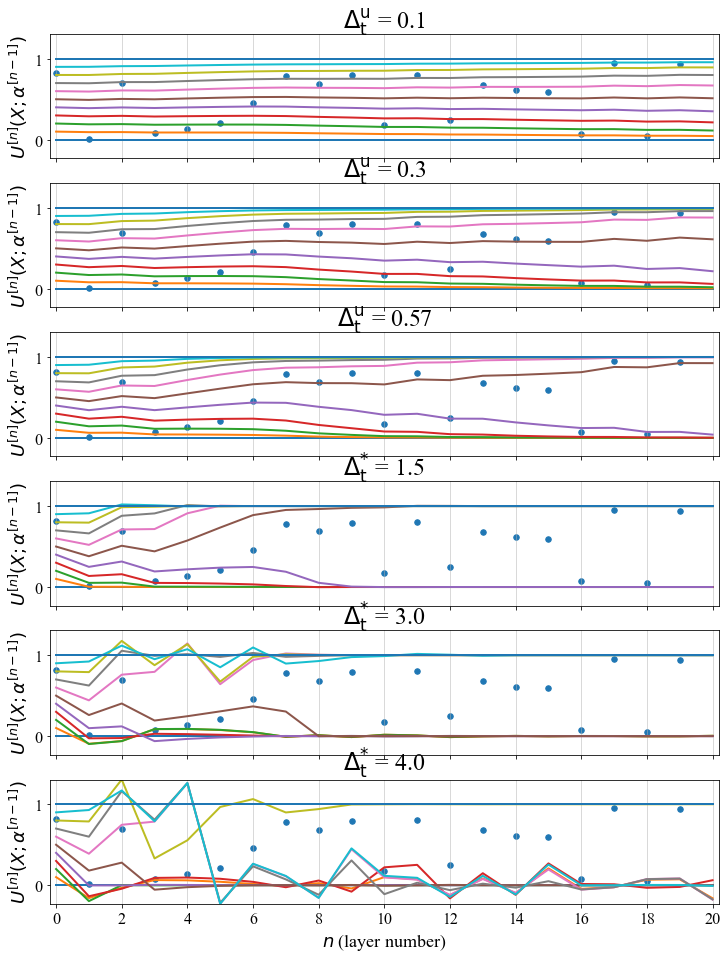
\includegraphics{figures/output_16_0.png}

The reasoning behind the existence of critical values of \(\mathrm{\Delta_{t}^u}\) under which the solution is ``well behaved'' (that is, the solution is always bounded) goes back to the idea of \emph{Invariant regions}, exploited extensively in PDEs: we refer the reader to Chapter 14 in \citep{Smoller}; if you want to see how it applies in the discrete setting, especially in finite-difference schemes for reaction diffusion models, see \citep{Hoff} and the Appendix C of the \href{https://arxiv.org/abs/2009.02467}{paper}).

\hypertarget{sec:1d}{%
\chapter{Applying the PSBC model to some toy problems}\label{sec:1d}}

We shall present the model in a simple toy problem, for illustrative purposes. As pointed out in the paper, we have to use a somewhat ``bigger''" model, of the form

\begin{equation} 
\begin{split}
U^{[n+1]} = U^{[n]} + \Delta_t^{u}\,f(U^{[n]},\alpha^{[n]}),\\
P^{[n+1]} = P^{[n]} + \Delta_t^{p}\,f(P^{[n]},\beta^{[n]}),
\end{split}\label{eq:4}
\end{equation}

where \(f(u,w):= u(1 - u)(u - w)\). Now, given a certain cost function that measures accuracy of the model (namely, how well it predicts in some examples) we have to train the model with respect to both variables \(\alpha^{[\cdot]}\) and \(\beta^{[\cdot]}\). What we see in \eqref{eq:4} is part of what we call Phase Separation Binary Classifier (PSBC). For now, we shall see how it behaves in the 1D model; in Section \ref{sec:mnist}, after many variations over this equation, we shall apply the model to the MNIST dataset.

\hypertarget{the-1d-rectangular-box-problem}{%
\section{The 1D Rectangular box problem}\label{the-1d-rectangular-box-problem}}

We shall work with a simple 1D model (the rectangular box problem), with the following labeling method:

\begin{equation}
Y =Y(X) = \left\{\begin{array}{cc} 1, & \text{if}\quad X \geq \gamma; \\ 
            0, & \text{otherwise}.
\end{array}\right.\label{eq:5}
\end{equation}

\begin{Shaded}
\begin{Highlighting}[]
\NormalTok{folder }\OperatorTok{=} \StringTok{"Statistics/MNIST/"}
\ControlFlowTok{with} \BuiltInTok{open}\NormalTok{(folder }\OperatorTok{+} \StringTok{"parameters_MNIST_Neumann.p"}\NormalTok{, }\StringTok{'rb'}\NormalTok{) }\ImportTok{as}\NormalTok{ fp: data }\OperatorTok{=}\NormalTok{ pickle.load(fp)}
\end{Highlighting}
\end{Shaded}

\begin{Shaded}
\begin{Highlighting}[]
\CommentTok{### GENERATE DATA}
\NormalTok{gamma, N_data }\OperatorTok{=} \FloatTok{.2}\NormalTok{, }\DecValTok{2000}
\NormalTok{X }\OperatorTok{=}\NormalTok{ np.reshape(np.random.uniform(}\DecValTok{0}\NormalTok{, }\DecValTok{1}\NormalTok{, N_data),(}\DecValTok{1}\NormalTok{, }\DecValTok{-1}\NormalTok{))}
\NormalTok{Y }\OperatorTok{=}\NormalTok{ np.array(X }\OperatorTok{>=}\NormalTok{ gamma, np.}\BuiltInTok{int}\NormalTok{, ndmin }\OperatorTok{=} \DecValTok{2}\NormalTok{)}

\CommentTok{### SPLIT DATA FOR CROSS VALIDATION}
\NormalTok{A, B, C, D }\OperatorTok{=}\NormalTok{ train_test_split(X.T, Y.T, test_size }\OperatorTok{=} \FloatTok{0.2}\NormalTok{)}
\CommentTok{#### We shall save one individual per column. We need to change that upon reading the csv later on}
\NormalTok{X_train, X_test, Y_train, Y_test }\OperatorTok{=}\NormalTok{ A.T, B.T, C.T, D.T}
\end{Highlighting}
\end{Shaded}

In this model, the data has to satisfy features dimension X number of elements in the sample

\begin{Shaded}
\begin{Highlighting}[]
\NormalTok{np.shape(X_train)}
\end{Highlighting}
\end{Shaded}

\(>>>\)

\begin{verbatim}
  (1, 1600)
\end{verbatim}

Things go more or less as before: we define the model's parameters,

\begin{Shaded}
\begin{Highlighting}[]
\NormalTok{learning_rate }\OperatorTok{=}\NormalTok{ (.}\DecValTok{1}\NormalTok{,.}\DecValTok{08}\NormalTok{,.}\DecValTok{93}\NormalTok{)}
\NormalTok{patience }\OperatorTok{=} \BuiltInTok{float}\NormalTok{(}\StringTok{"inf"}\NormalTok{)}
\NormalTok{sigma }\OperatorTok{=} \FloatTok{.1}
\NormalTok{drop_SGD }\OperatorTok{=} \FloatTok{0.95}  \CommentTok{# See  docstring of class "Binary_phase_separation" for further information}
\NormalTok{epochs, dt, dx, eps, Nx, Nt }\OperatorTok{=} \DecValTok{600}\NormalTok{, }\FloatTok{.1}\NormalTok{, }\DecValTok{1}\NormalTok{, }\DecValTok{0}\NormalTok{, }\DecValTok{1}\NormalTok{, }\DecValTok{20}
\NormalTok{weights_k_sharing }\OperatorTok{=}\NormalTok{ Nt}
\NormalTok{ptt_cardnlty }\OperatorTok{=} \DecValTok{1}
\NormalTok{batch_size }\OperatorTok{=} \VariableTok{None}
\NormalTok{subordinate, save_parameter_hist, orthodox_dt, with_phase }\OperatorTok{=} \VariableTok{True}\NormalTok{, }\VariableTok{True}\NormalTok{, }\VariableTok{True}\NormalTok{, }\VariableTok{True}
\end{Highlighting}
\end{Shaded}

and initialize the model

\begin{Shaded}
\begin{Highlighting}[]
\NormalTok{Init }\OperatorTok{=}\NormalTok{ Initialize_parameters()   }

\NormalTok{data }\OperatorTok{=}\NormalTok{ Init.dictionary(Nx, eps, dt, dx, Nt, ptt_cardnlty, weights_k_sharing, sigma }\OperatorTok{=}\NormalTok{ sigma )}
\NormalTok{data.update(\{}\StringTok{'learning_rate'}\NormalTok{ :  learning_rate, }\StringTok{'epochs'}\NormalTok{ :  epochs,}\OperatorTok{\textbackslash{}}
             \StringTok{'subordinate'}\NormalTok{ :  subordinate,}\StringTok{"patience"}\NormalTok{ : patience,}\OperatorTok{\textbackslash{}}
             \StringTok{'drop_SGD'}\NormalTok{ : drop_SGD,}\StringTok{"orthodox_dt"}\NormalTok{ : orthodox_dt,}\StringTok{'with_phase'}\NormalTok{ : with_phase,}
             \StringTok{"batch_size"}\NormalTok{ : batch_size, }\StringTok{"save_parameter_hist"}\NormalTok{ : save_parameter_hist \})}
\end{Highlighting}
\end{Shaded}

We are finally ready to train the model. We do so using the class Binary\_Phase\_Separation

\begin{Shaded}
\begin{Highlighting}[]
\NormalTok{Model }\OperatorTok{=}\NormalTok{ Binary_Phase_Separation()}
\end{Highlighting}
\end{Shaded}

Of which you can learn more about by typing

\begin{Shaded}
\begin{Highlighting}[]
\BuiltInTok{print}\NormalTok{(Model.__doc__)}
\end{Highlighting}
\end{Shaded}

\(>>>\)

\begin{verbatim}
   This is the main class  of the Phase Separation Binary Classifier (PSBC).
   With its methods one can, aong other things, train the model and 
   predict classifications (once the model has been trained).
\end{verbatim}

If the above is not enough, you can type

\begin{Shaded}
\begin{Highlighting}[]
\BuiltInTok{print}\NormalTok{(}\BuiltInTok{help}\NormalTok{(Model))}
\end{Highlighting}
\end{Shaded}

\(>>>\)

\begin{verbatim}
Help on Binary_Phase_Separation in module binary_phase_separation object:

class Binary_Phase_Separation(builtins.object)
 |  Binary_Phase_Separation(cost=None, par_U_model=None, par_P_model=None, par_U_wrt_epochs=None, par_P_wrt_epochs=None)
 |  
...
\end{verbatim}

But this is maybe too much. So, let's say that you just want to know about how to train. You can get information only about that method

\begin{Shaded}
\begin{Highlighting}[]
\BuiltInTok{print}\NormalTok{(Model.train.__doc__)}
\end{Highlighting}
\end{Shaded}

\(>>>\)

\begin{verbatim}
        'train' method.

        This method trains the PSBC model with a given set of parameters and 
        data.
        
        Parameters
        ----------
        X : numpy.ndarray of size Nx X N_data
            Matrix with features. 
        ...    
\end{verbatim}

The method that we want is train. So, we do

\begin{Shaded}
\begin{Highlighting}[]
\NormalTok{Model.train(}
\NormalTok{    X_train, Y_train, X_train, Y_train, learning_rate, dt, dx, Nt,}\OperatorTok{\textbackslash{}}
\NormalTok{        weights_k_sharing, eps }\OperatorTok{=}\NormalTok{ eps, epochs }\OperatorTok{=}\NormalTok{ epochs, }\OperatorTok{\textbackslash{}}
\NormalTok{        subordinate }\OperatorTok{=}\NormalTok{ subordinate, with_phase }\OperatorTok{=}\NormalTok{ with_phase,}\OperatorTok{\textbackslash{}}
\NormalTok{        drop_SGD }\OperatorTok{=}\NormalTok{ drop_SGD, sigma }\OperatorTok{=}\NormalTok{ sigma,}\OperatorTok{\textbackslash{}}
\NormalTok{        orthodox_dt }\OperatorTok{=}\NormalTok{ orthodox_dt, print_every }\OperatorTok{=} \DecValTok{300}\NormalTok{,}\OperatorTok{\textbackslash{}}
\NormalTok{            save_parameter_hist }\OperatorTok{=}\NormalTok{ save_parameter_hist}
\NormalTok{)}
\end{Highlighting}
\end{Shaded}

\(>>>\)

\begin{verbatim}
 epoch : 0 cost 0.11494985702898435

 accuracy : 0.70375

 epoch : 300 cost 0.022553932287346947

 accuracy : 0.9775
\end{verbatim}

If you want to take a look at how the cost function behaves over epochs, you can plot it (see full code in \href{https://github.com/rafael-a-monteiro-math/Binary_classification_phase_separation/blob/master/Notebook_PSBC_examples.ipynb}{Notebook\_examples.ipynb}). The output is given below.

\begin{figure}[htbp]
\centering
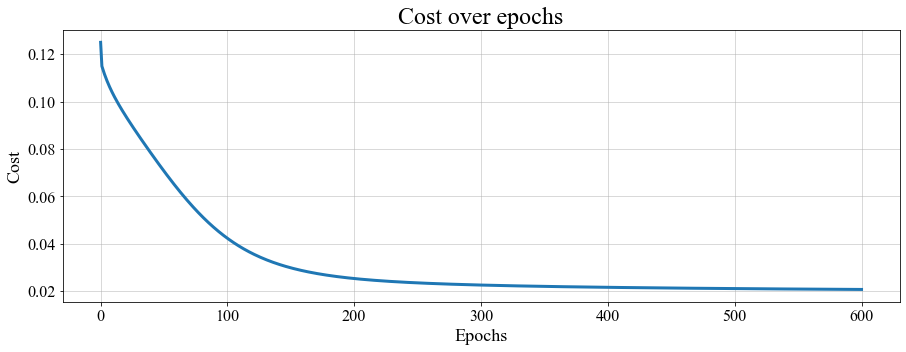
\includegraphics[width=0.9\textwidth,height=\textheight]{figures/output_37_0.png}
\caption{The evolution of the cost over epochs, for the 1D PSBC model with labeling \ref{eq:5}.}
\end{figure}
And if you want to take a look at the behavior of the set \(\mathscr{P}_{\alpha}\) you can also do. Just type

\begin{Shaded}
\begin{Highlighting}[]
\NormalTok{diameter_history }\OperatorTok{=}\NormalTok{ Model.diameters_hist}
\end{Highlighting}
\end{Shaded}

which will give you a dictionary with two keys: ``U'' and ``P''

\begin{Shaded}
\begin{Highlighting}[]
\NormalTok{diameter_history.keys()}
\end{Highlighting}
\end{Shaded}

\(>>>\)

\begin{verbatim}
dict_keys(['P', 'U'])
\end{verbatim}

They concern the behavior of trainable weights for the U variable, and for the P variable. They can be plotted as
\begin{figure}[htbp]
\centering
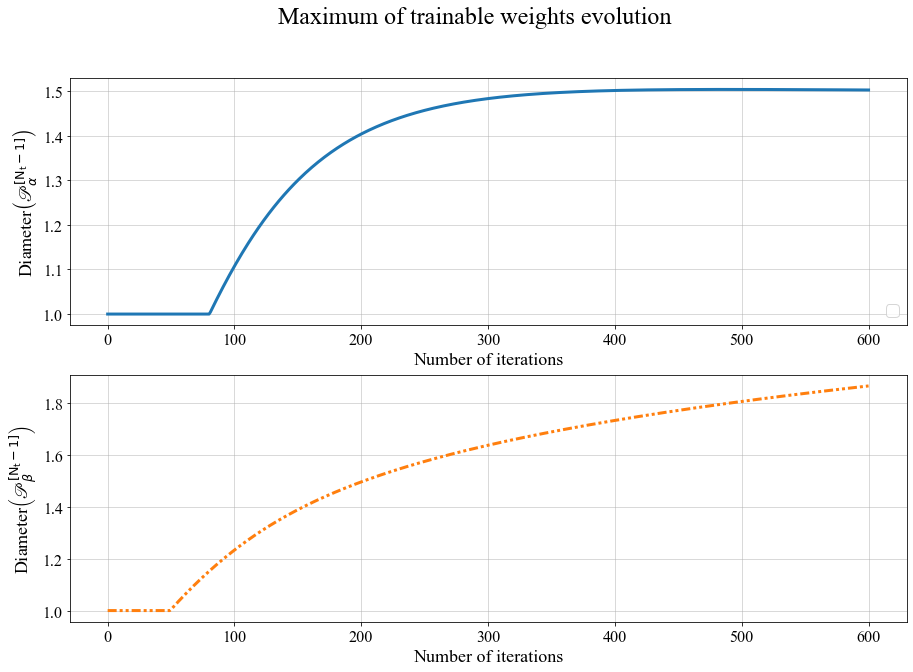
\includegraphics[width=0.8\textwidth]{figures/output_43_1.png}
\caption{The evolution of the diameters $\mathscr{P}_{\alpha}$ and $\mathscr{P}_{\beta}$ over epochs, for the 1D PSBC model with labeling \ref{eq:5}.}
\end{figure}

This is the typical behavior of these quantities: they remain constant (equal to 1) up to a certain point, to then grow in a logarithmic shape. Note that the point of departure from the value 1 is different for both variables; that's because both quantities \(\Delta_t^u\) and \(\Delta_t^p\) in \eqref{eq:4} are allowed to vary independently (see the \href{https://arxiv.org/abs/2009.02467}{paper} for further information).

We can also check the behavior of accuracythroughout epochs:

\begin{figure}[htbp]
\centering
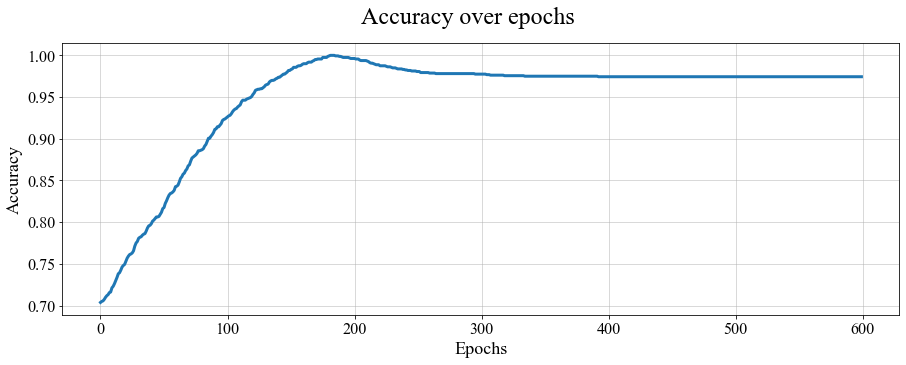
\includegraphics[width=0.9\textwidth]{figures/output_45_0.png}
\caption{The evolution of accuracy over epochs, for the 1D PSBC modelwith labeling \ref{eq:5}.}
\end{figure}
Note the the model peaks (reaches a point of high accuracy) before the final epoch. This natural ``deterioration'' is what lead researchers to design \textbf{Early Stopping} methods; cf.~\citep{early_when}. We can in fact know what that epoch was by typing

\begin{Shaded}
\begin{Highlighting}[]
\NormalTok{Model.best_epoch}
\end{Highlighting}
\end{Shaded}

\(>>>\) 
\begin{verbatim}
array(181)
\end{verbatim}
\
which is before final epoch - in this case, 600. The accucary (for the training set) at epoch 181 was

\begin{Shaded}
\begin{Highlighting}[]
\NormalTok{Model.best_accuracy}
\end{Highlighting}
\end{Shaded}

\(>>>\) 
\begin{verbatim}
array(1.)
\end{verbatim}

that is, 100\% accuracy. If you want to retrieve the model parameters at such an epoch you just need to type

\begin{Shaded}
\begin{Highlighting}[]
\NormalTok{best_P , best_U }\OperatorTok{=}\NormalTok{ Model.best_par_P_model, Model.best_par_U_model}
\end{Highlighting}
\end{Shaded}

which will give the value of the parameters used when the model achieved its best performance.

For this simple model we did something else: we are saving all the parameters in the model at each epoch. \footnote{It is clear that whenever one deals with big models memory is an impeditive obstruction to reproducing this; in such a case, it is better to set ``save\_parameter\_hist = False'' in order to save memory.}

\begin{figure}[htbp]
\centering
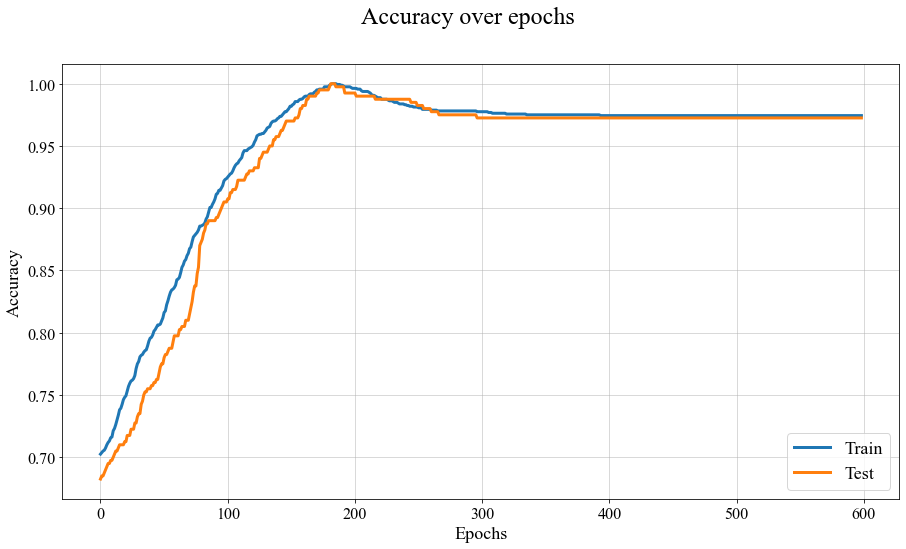
\includegraphics[width=0.9\textwidth,height=\textheight]{figures/output_55_0.png}
\caption{Evolution of accuracy for train and test set over epochs, for the 1D PSBC problem with labeling \ref{eq:5}}
\end{figure}

\hypertarget{sec:mnist}{%
\chapter{The MNIST database}\label{sec:mnist}}

The MNIST database is a well known database of handwritten digits used in the classical paper \citep{Mnist}. In this project we only used (suggestively) the subset of digits ``0'' and ``1'', for we are doing binary classification only.

\begin{Shaded}
\begin{Highlighting}[]
\CommentTok{### READ MNIST DATASET TO PANDAS DATAFRAME AND THEN TO NUMPY FILE}
\NormalTok{data_train_MNIST }\OperatorTok{=}\NormalTok{ pd.read_csv(}\StringTok{'Examples/data_train_normalized_MNIST.csv'}\NormalTok{)}
\NormalTok{data_test_MNIST }\OperatorTok{=}\NormalTok{ pd.read_csv(}\StringTok{'Examples/data_test_normalized_MNIST.csv'}\NormalTok{)}
\end{Highlighting}
\end{Shaded}

\begin{Shaded}
\begin{Highlighting}[]
\NormalTok{X_train_MNIST }\OperatorTok{=}\NormalTok{ (data_train_MNIST.iloc[:,:}\OperatorTok{-}\DecValTok{1}\NormalTok{]).to_numpy()}
\NormalTok{Y_train_MNIST }\OperatorTok{=}\NormalTok{ np.reshape(data_train_MNIST.iloc[:,}\OperatorTok{-}\DecValTok{1}\NormalTok{].to_numpy(), (}\DecValTok{1}\NormalTok{,}\OperatorTok{-}\DecValTok{1}\NormalTok{))}
\NormalTok{X_test_MNIST }\OperatorTok{=}\NormalTok{ (data_test_MNIST.iloc[:,:}\OperatorTok{-}\DecValTok{1}\NormalTok{]).to_numpy()}
\NormalTok{Y_test_MNIST }\OperatorTok{=}\NormalTok{ np.reshape(data_test_MNIST.iloc[:,}\OperatorTok{-}\DecValTok{1}\NormalTok{].to_numpy(), (}\DecValTok{1}\NormalTok{,}\OperatorTok{-}\DecValTok{1}\NormalTok{))}

\NormalTok{X_train_MNIST, X_test_MNIST }\OperatorTok{=}\NormalTok{ X_train_MNIST.T , X_test_MNIST.T}
\end{Highlighting}
\end{Shaded}

\begin{figure}[htbp]
\centering
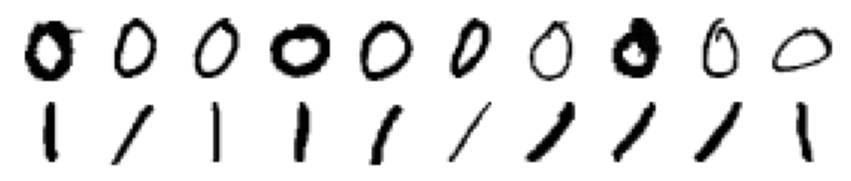
\includegraphics{figures/output_63_0.png}
\caption{A  subsample of digits "0" and "1" in the MNIST database.}
\end{figure}

One can also visualize the trainable weights as heatmaps (see full code in \href{https://github.com/rafael-a-monteiro-math/Binary_classification_phase_separation/blob/master/Notebook_PSBC_examples.ipynb}{Notebook\_examples.ipynb}).

\begin{figure}[htbp]
\centering
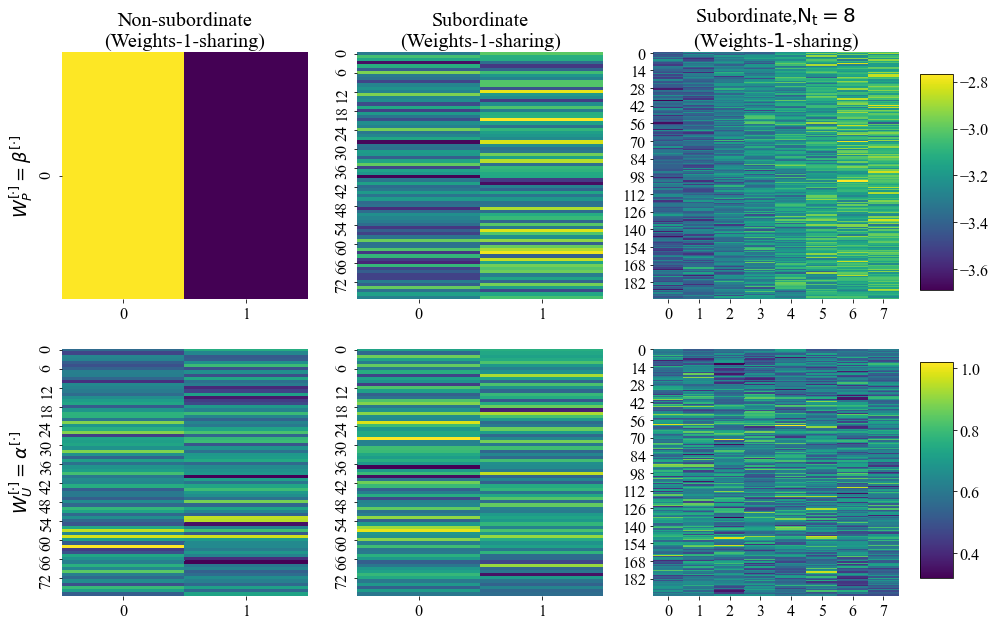
\includegraphics{figures/output_67_0.png}
\caption{Heatmaps of trainable weights for some trained PSBC models in the Examples folder.}
\end{figure}

\hypertarget{retrieving-some-statistics}{%
\section{Retrieving some statistics}\label{retrieving-some-statistics}}

To get a flavor of what is in the statistics folder, we first need to retrieve some of this data:

\begin{Shaded}
\begin{Highlighting}[]
\NormalTok{parameters_MNIST_nondif, stats_folder_MNIST }\OperatorTok{=}\NormalTok{ \{\}, }\StringTok{"Statistics/MNIST/"}
\ControlFlowTok{with} \BuiltInTok{open}\NormalTok{(stats_folder_MNIST }\OperatorTok{+} \StringTok{"parameters_MNIST_nondif.p"}\NormalTok{, }\StringTok{'rb'}\NormalTok{) }\ImportTok{as}\NormalTok{ fp: }
\NormalTok{    parameters_MNIST_nondif }\OperatorTok{=}\NormalTok{ pickle.load(fp)}

\NormalTok{parameters_MNIST_Neumann, stats_folder_MNIST }\OperatorTok{=}\NormalTok{ \{\}, }\StringTok{"Statistics/MNIST/"}
\ControlFlowTok{with} \BuiltInTok{open}\NormalTok{(stats_folder_MNIST }\OperatorTok{+} \StringTok{"parameters_MNIST_Neumann.p"}\NormalTok{, }\StringTok{'rb'}\NormalTok{) }\ImportTok{as}\NormalTok{ fp:}
\NormalTok{        parameters_MNIST_Neumann }\OperatorTok{=}\NormalTok{ pickle.load(fp)}

\NormalTok{parameters_MNIST_Periodic, stats_folder_MNIST }\OperatorTok{=}\NormalTok{ \{\}, }\StringTok{"Statistics/MNIST/"}
\ControlFlowTok{with} \BuiltInTok{open}\NormalTok{(stats_folder_MNIST }\OperatorTok{+} \StringTok{"parameters_MNIST_Periodic.p"}\NormalTok{, }\StringTok{'rb'}\NormalTok{) }\ImportTok{as}\NormalTok{ fp:}
\NormalTok{        parameters_MNIST_Periodic }\OperatorTok{=}\NormalTok{ pickle.load(fp)}
\end{Highlighting}
\end{Shaded}

The function \emph{accuracies} is part of the module \emph{aux\_fnts\_for\_jupyter\_notebooks.py}, which is available in this Github \citep{Bin_phase_github}. As before, help on this equation can be called typing `help(accuracies)'.

With data in the Statistics folder we can plot the graph of accuracies of the non-diffusive PSBC for different values of partition cardinality \(\mathrm{N_{ptt}}\).

\begin{figure}[htbp]
\centering
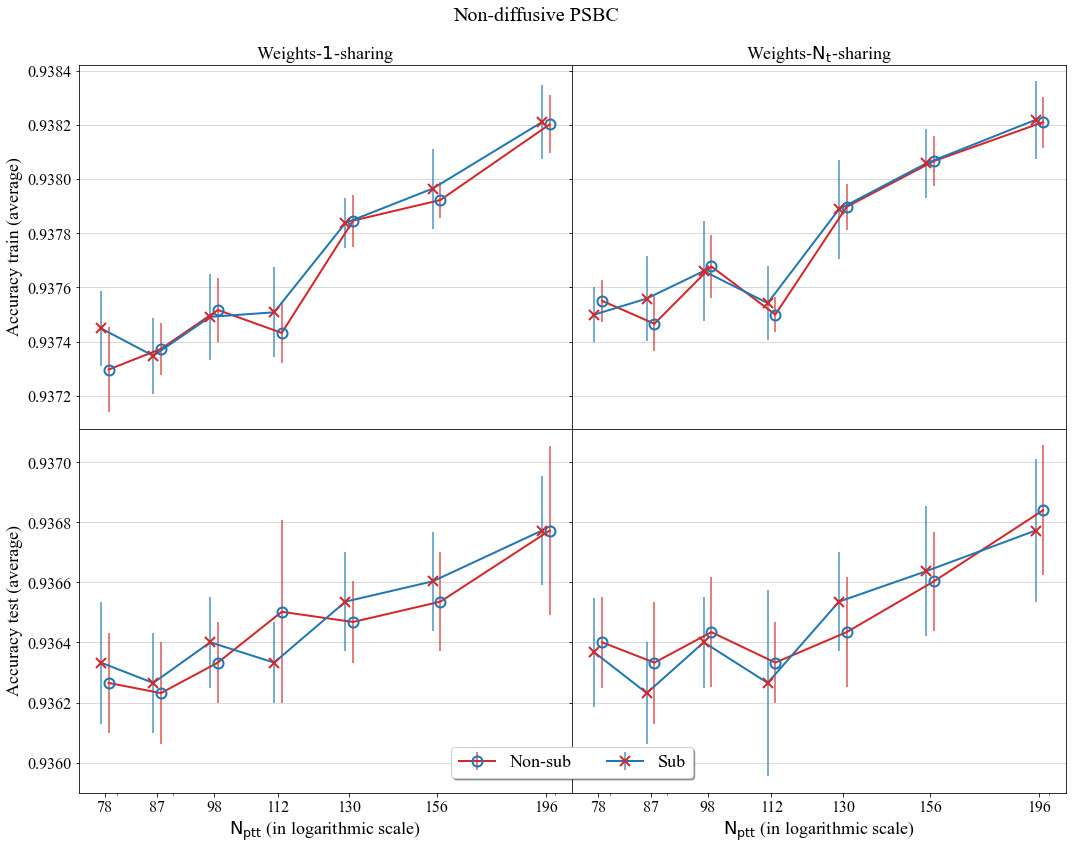
\includegraphics[width=0.9\textwidth,height=\textheight]{figures/output_72_0.png}
\caption{A comparison of average accuracy of the non-diffusive PSBC for different values of Partition cardinality; models compared either have subordinate phase (tagged as "Sub") or not (non-subordinate phase, tagged as "Non-sub").}
\end{figure}
If can also see the evolution of the maximum of trainable weights over epochs, for a Periodic PSBC with \(\mathrm{N_t} =1\).

\begin{figure}[htbp]
\centering
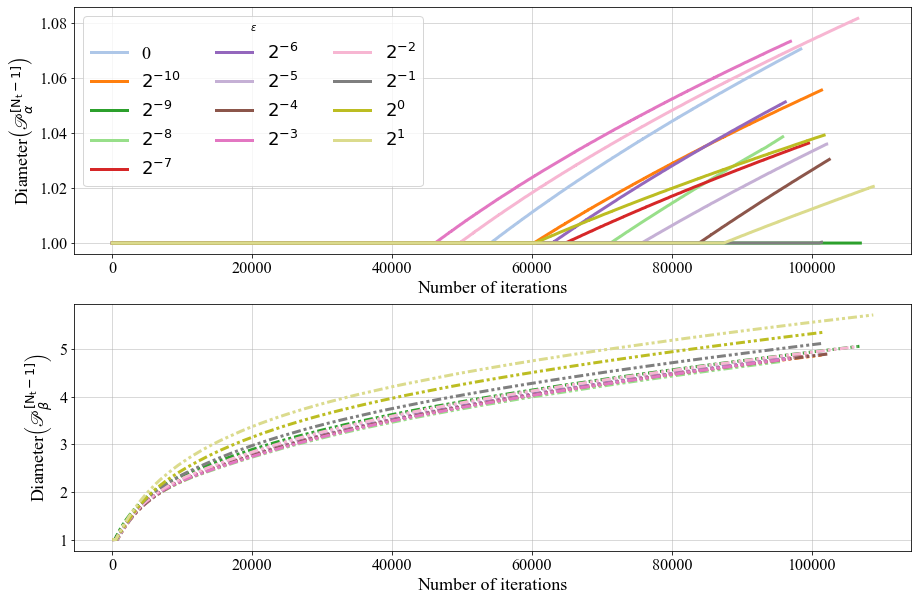
\includegraphics[width=0.8\textwidth,height=\textheight]{figures/output_75_1.png}
\caption{The behavior of $\mathscr{P}_{\alpha}^{[\cdot]}$ and $\mathscr{P}_{\beta}^{[\cdot]}$ over time, for a Periodic PSBC with $\mathrm{N_t} =1$.}
\end{figure}

With these data we can also plot confusion matrices.

\begin{Shaded}
\begin{Highlighting}[]
\NormalTok{parent_folder }\OperatorTok{=} \StringTok{"Examples/"}
\NormalTok{folder_now }\OperatorTok{=}\NormalTok{ parent_folder }\OperatorTok{+} \StringTok{"W1S-Nt8/simulation1/"}
\ControlFlowTok{with} \BuiltInTok{open}\NormalTok{(folder_now }\OperatorTok{+} \StringTok{"Full_model_properties.p"}\NormalTok{, }\StringTok{'rb'}\NormalTok{) }\ImportTok{as}\NormalTok{ fp:}
\NormalTok{	Full_model_properties }\OperatorTok{=}\NormalTok{ pickle.load(fp)}
\end{Highlighting}
\end{Shaded}

\begin{figure}[htbp]
\centering
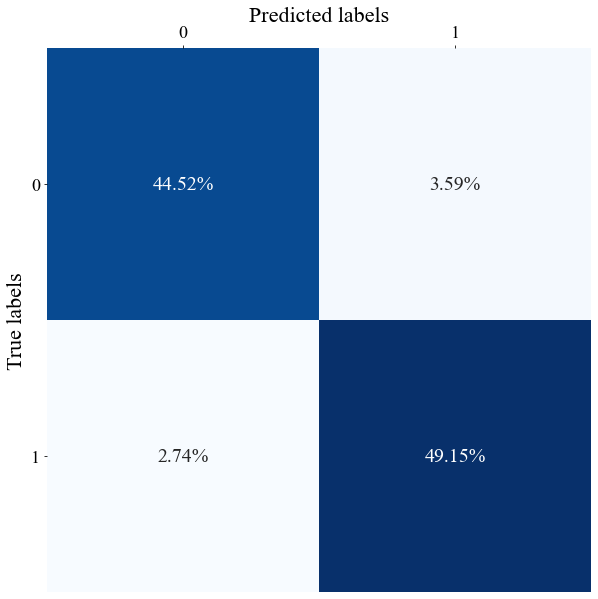
\includegraphics[width=0.5\textwidth]{figures/output_80_0.png}
\caption{Confusion matrix of  a realization of the diffusive PSBC with Neumann BCs, weights-1-sharing, and $\mathrm{N_t = 8}$.}
\end{figure}

There are other things that we do as well: for instance, we can plot Table 4 in the \href{https://github.com/rafael-a-monteiro-math/Binary_classification_phase_separation/blob/master/Supplement.pdf}{Supplement}, which shows the average value of the maximum (in \(\ell^{\infty}\)-norm) of trainable weights of non-diffusive PSBC models for different values of partition cardinality \(\mathrm{N_t}\).

\begin{figure}[htbp]
\centering
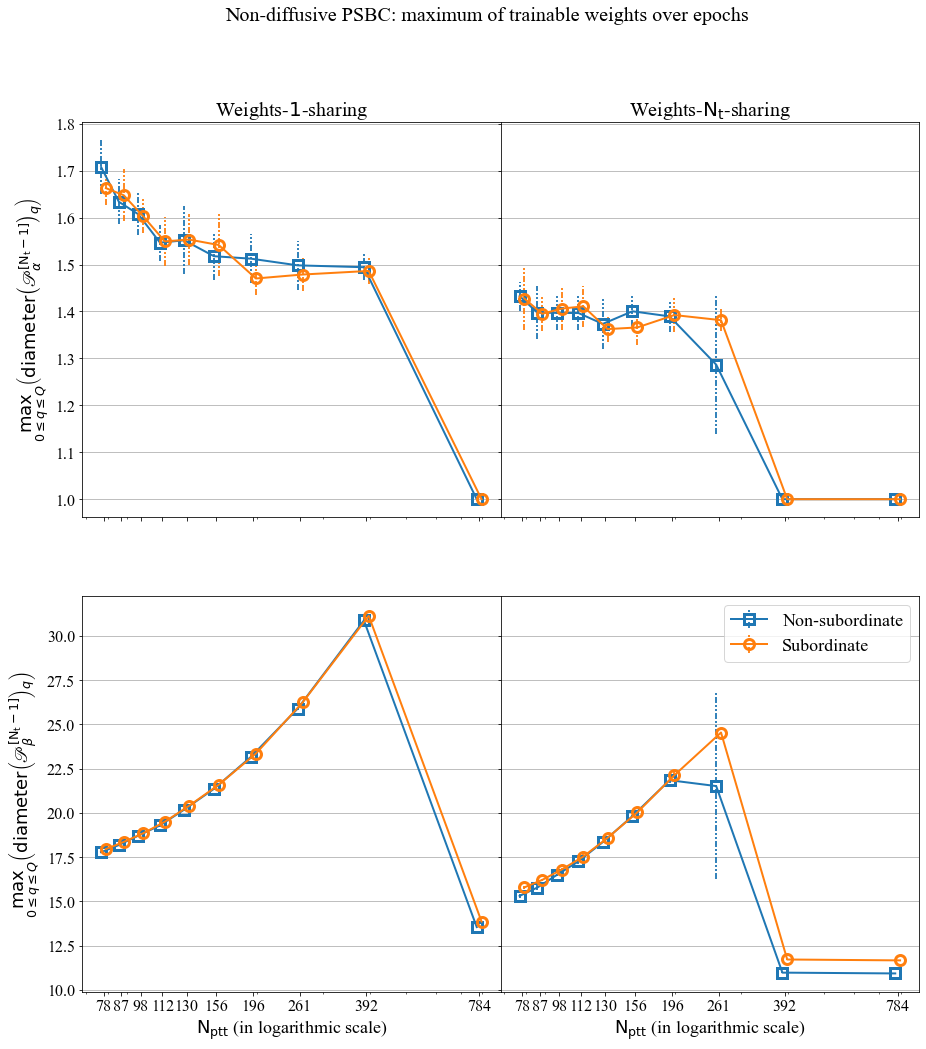
\includegraphics[width=0.8\textwidth]{figures/max_non-dif.png}
\caption{The maximum over epochs. You find the code for this plot in \href{https://github.com/rafael-a-monteiro-math/Binary_classification_phase_separation/blob/master/Notebook_PSBC_examples.ipynb}{Notebook\_examples.ipynb}}
\end{figure}


\hypertarget{a-homemade-example-hadwritten-0-and-1}{%
\section{A ``homemade'' example: hadwritten 0 and 1}\label{a-homemade-example-hadwritten-0-and-1}}

We now step foward to a higher dimensional feature space, using equations that are similar to those shown in Section \ref{sec:1d} of this tutorial. There is an interesting interplay between high-dimensionality of feature spaces and model compressibility, which we highlight here by applying the PSBC to the subset ``0''-``1'' of the MNIST database; we once more refer the reader to Sections 4 and 5 in the \href{https://arxiv.org/abs/2009.02467}{paper} for more details.

The goal in this section is to illustrate a bit more of the PSBC's use by predicting the label for some of the author's own handwritten numbers. For that we shall use the trainable models available in \citep{Bin_phase_data}, in the tarball \textbf{PSBC\_Examples.tar.gz}. Two of these digits are shown below.

\begin{figure}[htbp]
\centering
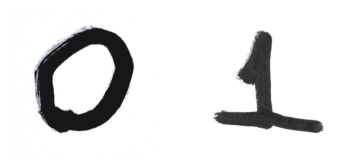
\includegraphics{figures/output_85_0.png}
\caption{Two of the author's own handwritten numbers; original photo, treated using Gimp.}
\end{figure}

In fact, we shall use 6 of the author's handwritten digits - 3 zeros, 3 ones - for this notebook. If you read the first papers of LeCun et al.~about the MNIST project, there is a description of the way pictures were taken (see for instance, Section III A in \citep{Mnist}, or the explanation in \href{http://yann.lecun.com/exdb/mnist/}{LeCun's MNIST webpage}), so that they look the way they do in cell 36 of \href{https://github.com/rafael-a-monteiro-math/Binary_classification_phase_separation/blob/master/Notebook_PSBC_examples.ipynb}{Notebook\_examples.ipynb}: the images had to be controlled for angle, centralization, etc; this is part of the statistical design, which I tried to follow here without too much concern (because this is just a tutorial) but, somehow, ``as close as possible''.

Pictures we cropped using \href{https://www.gimp.org}{GIMP}, a free software for image manipulation: you take a picture, crop it, go to image, set it into grayscale, adjust for light contrast and other things. And that's it.

Now, with them cropped, ``MNIST-like'' grayscale images in hands, you proceed as in the next cell, reshaping these pictures as a 28 x 28 matrix. We show what the two digits that you saw before will look like.

\begin{Shaded}
\begin{Highlighting}[]
\ImportTok{from}\NormalTok{ PIL }\ImportTok{import}\NormalTok{ Image}

\KeywordTok{def}\NormalTok{ create_MNIST_type_figure(name):}
    \CommentTok{"""Convert jpg figure to a (28,28) numpy array"""}
\NormalTok{    image }\OperatorTok{=}\NormalTok{ Image.}\BuiltInTok{open}\NormalTok{(name).convert(}\StringTok{'L'}\NormalTok{)}
\NormalTok{    image2 }\OperatorTok{=}\NormalTok{ image.resize((}\DecValTok{28}\NormalTok{,}\DecValTok{28}\NormalTok{))}
\NormalTok{    im2_as_array }\OperatorTok{=} \DecValTok{255}\OperatorTok{-}\NormalTok{ np.array(image2,  dtype}\OperatorTok{=}\NormalTok{np.uint8)}
    \BuiltInTok{print}\NormalTok{(}\StringTok{"image has shape"}\NormalTok{, im2_as_array.shape)}

    \ControlFlowTok{return}\NormalTok{ im2_as_array}

\NormalTok{my_0 }\OperatorTok{=}\NormalTok{ create_MNIST_type_figure(}\StringTok{"figures/my_0.jpg"}\NormalTok{)}
\NormalTok{my_0_v2 }\OperatorTok{=}\NormalTok{ create_MNIST_type_figure(}\StringTok{"figures/my_0_v2.jpg"}\NormalTok{)}
\NormalTok{my_0_v3 }\OperatorTok{=}\NormalTok{ create_MNIST_type_figure(}\StringTok{"figures/my_0_v3.jpg"}\NormalTok{)}
\NormalTok{my_1 }\OperatorTok{=}\NormalTok{ create_MNIST_type_figure(}\StringTok{"figures/my_1.jpg"}\NormalTok{)}
\NormalTok{my_1_v2 }\OperatorTok{=}\NormalTok{ create_MNIST_type_figure(}\StringTok{"figures/my_1_v2.jpg"}\NormalTok{)}
\NormalTok{my_1_v3 }\OperatorTok{=}\NormalTok{ create_MNIST_type_figure(}\StringTok{"figures/my_1_v3.jpg"}\NormalTok{)}

\NormalTok{fig, ax }\OperatorTok{=}\NormalTok{ plt.subplots(}\DecValTok{1}\NormalTok{,}\DecValTok{2}\NormalTok{)}
\NormalTok{ax[}\DecValTok{0}\NormalTok{].imshow(my_0, cmap}\OperatorTok{=}\StringTok{'binary'}\NormalTok{)}
\NormalTok{ax[}\DecValTok{1}\NormalTok{].imshow(my_1, cmap}\OperatorTok{=}\StringTok{'binary'}\NormalTok{)}
\NormalTok{ax[}\DecValTok{0}\NormalTok{].axis(}\VariableTok{False}\NormalTok{)}
\NormalTok{ax[}\DecValTok{1}\NormalTok{].axis(}\VariableTok{False}\NormalTok{)}
\NormalTok{plt.show()}
\end{Highlighting}
\end{Shaded}

You will get this

\begin{figure}[htbp]
\centering

\includegraphics{figures/output_87_1.png}
\caption{The handwritten digits shown above, now as 28X28 pixels images.}
\end{figure}
Recall that we need to flatten these matrices,

\begin{Shaded}
\begin{Highlighting}[]
\NormalTok{my_0_for_psbc }\OperatorTok{=}\NormalTok{ my_0.flatten(order}\OperatorTok{=}\StringTok{'C'}\NormalTok{)}
\NormalTok{...}
\end{Highlighting}
\end{Shaded}

and we can then combine all these 6 flattened images as columns in a single matrix \textbf{combined\_handwritten}, whose size is \(784\times 6\).

Now we initialize the PSBC model

\begin{Shaded}
\begin{Highlighting}[]
\ControlFlowTok{with} \BuiltInTok{open}\NormalTok{(}\StringTok{"Examples/W1S-Nt8/simulation1/Full_model_properties.p"}\NormalTok{, }\StringTok{'rb'}\NormalTok{) }\ImportTok{as}\NormalTok{ fp:}
\NormalTok{	load_mnist }\OperatorTok{=}\NormalTok{ pickle.load(fp)}

\NormalTok{psbc_testing }\OperatorTok{=}\NormalTok{ Binary_Phase_Separation()}
\end{Highlighting}
\end{Shaded}

and apply to our matrix/data \textbf{combined\_handwritten} with the trained weights we have chosen.

\begin{Shaded}
\begin{Highlighting}[]
\NormalTok{prediction }\OperatorTok{=}\NormalTok{ psbc_testing.predict(combined_handwritten, load_mnist[}\StringTok{"best_par_U_model"}\NormalTok{],}
\NormalTok{	load_mnist[}\StringTok{"best_par_P_model"}\NormalTok{])}
\BuiltInTok{print}\NormalTok{(prediction)}
\end{Highlighting}
\end{Shaded}

\ldots and we fail, as we see in the output below. Floating number overflows, ``NAN'', etc.. sad news..

\(>>>\)

\begin{verbatim}
[0 0 0 0 0 0]

/Users/rafaelmonteiro/Desktop/PSBC/All_cases/binary_phase_separation.py:475: 
		RuntimeWarning: overflow encountered in multiply
  v = v +  dt * v * (1-v) * (v-alpha_x_t)
/Users/rafaelmonteiro/Desktop/PSBC/All_cases/binary_phase_separation.py:477: 
		RuntimeWarning: invalid value encountered in matmul
  v = np.matmul(Minv,v)
/Users/rafaelmonteiro/Desktop/PSBC/All_cases/binary_phase_separation.py:1128: 
		RuntimeWarning: invalid value encountered in greater
  keepdims = True, axis = 0))) > .5, dtype = np.int32)
\end{verbatim}

This seems really bad\ldots{} but do not despair: recall that data need to satisfy the \textbf{normalization conditions}: all the features have to be in the range \([0,1]\). We are in fact very far from that now: if you look for the minimum and maximum value of these matrices you will get \(0\) and \(255\), respectively, as an answer.

With that said, let's normalize the data:

\begin{Shaded}
\begin{Highlighting}[]
\NormalTok{init_data }\OperatorTok{=}\NormalTok{ Initialize_Data()}
\end{Highlighting}
\end{Shaded}

So, the data get's normalized, but centered. By default, it gets rescaled in the range {[}0.4,0.6{]}. What we do then is: (i) we normalize it, then (ii) we add 0.1 to it.

\begin{Shaded}
\begin{Highlighting}[]
\NormalTok{combined_handwritten_for_psbc, _, _ }\OperatorTok{=}\NormalTok{ init_data.normalize(combined_handwritten)}
\NormalTok{combined_handwritten_for_psbc }\OperatorTok{=} \FloatTok{0.1}\OperatorTok{+}\NormalTok{ combined_handwritten_for_psbc}
\end{Highlighting}
\end{Shaded}

Now we are in better shape: if you look for minimum and maximum of the matrix \(combined\_handwritten\_for\_psbc\) you will get \(0.5\) and \(0.7000000000000001\).

\begin{figure}[htbp]
\centering

\includegraphics{figures/output_105_0.png}
\caption{Some of the author's handwritten examples for this tutorial.}
\end{figure}
Now let's see how well the PSBC does in predicting them (note that, for the subset ``0'' and ``1'' of the MNIST database we already know that all these model perform quite well, separating these two classes with accuracy about 94\%).

\begin{Shaded}
\begin{Highlighting}[]
\ControlFlowTok{for}\NormalTok{ name }\KeywordTok{in}\NormalTok{ [}\StringTok{"W1S-NS"}\NormalTok{, }\StringTok{"W1S-S"}\NormalTok{, }\StringTok{"WNtS-NS"}\NormalTok{, }\StringTok{"WNtS-S"}\NormalTok{,}\OperatorTok{\textbackslash{}}
            \StringTok{"W1S-Nt2"}\NormalTok{, }\StringTok{"W1S-Nt4"}\NormalTok{, }\StringTok{"W1S-Nt8"}\NormalTok{,}\OperatorTok{\textbackslash{}}
             \StringTok{"WNtS-Nt1"}\NormalTok{,}\StringTok{"WNtS-Nt2"}\NormalTok{, }\StringTok{"WNtS-Nt4"}\NormalTok{, }\StringTok{"WNtS-Nt8"}\NormalTok{,}\OperatorTok{\textbackslash{}}
             \StringTok{"Per_W1S-Nt2"}\NormalTok{, }\StringTok{"Per_W1S-Nt4"}\NormalTok{, }\StringTok{"Per_W1S-Nt8"}\NormalTok{,}\OperatorTok{\textbackslash{}}
             \StringTok{"Per_WNtS-Nt1"}\NormalTok{,}\StringTok{"Per_WNtS-Nt2"}\NormalTok{, }\StringTok{"Per_WNtS-Nt4"}\NormalTok{, }\StringTok{"Per_WNtS-Nt8"}\NormalTok{]:}
            
    \ControlFlowTok{with} \BuiltInTok{open}\NormalTok{(}\StringTok{"Examples/"}\OperatorTok{+}\NormalTok{name}\OperatorTok{+}\StringTok{"/simulation1/Full_model_properties.p"}\NormalTok{, }\StringTok{'rb'}\NormalTok{) }\ImportTok{as}\NormalTok{ fp:}
\NormalTok{        load_mnist }\OperatorTok{=}\NormalTok{ pickle.load(fp)}
    
\NormalTok{    psbc_testing }\OperatorTok{=}\NormalTok{ Binary_Phase_Separation()}
\NormalTok{    prediction }\OperatorTok{=} \OperatorTok{\textbackslash{}}
\NormalTok{    psbc_testing.predict(}
\NormalTok{        combined_handwritten_for_psbc,  load_mnist[}\StringTok{"best_par_U_model"}\NormalTok{],}\OperatorTok{\textbackslash{}} 
\NormalTok{			load_mnist[}\StringTok{"best_par_P_model"}\NormalTok{],}\OperatorTok{\textbackslash{}}
\NormalTok{        subordinate }\OperatorTok{=}\NormalTok{ load_mnist[}\StringTok{"best_par_U_model"}\NormalTok{][}\StringTok{"subordinate"}\NormalTok{]}
\NormalTok{    )}
    \BuiltInTok{print}\NormalTok{(}\StringTok{"Model"}\NormalTok{, name, }\StringTok{" predicts"}\NormalTok{, np.squeeze(prediction), }\StringTok{"and correct is, [0 0 0 1 1 1]"}\NormalTok{ )}
\end{Highlighting}
\end{Shaded}

\(>>>\)

\begin{verbatim}
Model W1S-NS  predicts [0 0 0 0 1 1] and correct is, [0 0 0 1 1 1]
Model W1S-S  predicts [0 0 0 0 1 1] and correct is, [0 0 0 1 1 1]
Model WNtS-NS  predicts [0 0 0 0 1 1] and correct is, [0 0 0 1 1 1]
Model WNtS-S  predicts [0 0 0 0 1 1] and correct is, [0 0 0 1 1 1]
Model W1S-Nt2  predicts [0 0 0 0 1 1] and correct is, [0 0 0 1 1 1]
Model W1S-Nt4  predicts [0 0 0 0 1 1] and correct is, [0 0 0 1 1 1]
Model W1S-Nt8  predicts [0 0 0 0 1 1] and correct is, [0 0 0 1 1 1]
Model WNtS-Nt1  predicts [0 0 0 0 1 1] and correct is, [0 0 0 1 1 1]
Model WNtS-Nt2  predicts [0 0 0 0 1 1] and correct is, [0 0 0 1 1 1]
Model WNtS-Nt4  predicts [0 0 0 0 1 1] and correct is, [0 0 0 1 1 1]
Model WNtS-Nt8  predicts [0 0 0 0 1 1] and correct is, [0 0 0 1 1 1]
Model Per_W1S-Nt2  predicts [0 0 0 0 1 1] and correct is, [0 0 0 1 1 1]
Model Per_W1S-Nt4  predicts [0 0 0 0 1 1] and correct is, [0 0 0 1 1 1]
Model Per_W1S-Nt8  predicts [0 0 0 0 1 1] and correct is, [0 0 0 1 1 1]
Model Per_WNtS-Nt1  predicts [0 0 0 0 1 1] and correct is, [0 0 0 1 1 1]
Model Per_WNtS-Nt2  predicts [0 0 0 0 1 1] and correct is, [0 0 0 1 1 1]
Model Per_WNtS-Nt4  predicts [0 0 0 0 1 1] and correct is, [0 0 0 1 1 1]
Model Per_WNtS-Nt8  predicts [0 0 0 0 1 1] and correct is, [0 0 0 1 1 1]
\end{verbatim}

It is getting all correct, except for the 4th picture (which is in fact the way that I usually write, with that huge horizontal ``foot'').

\hypertarget{the-phase-separation-binary-classifier-where-to-read-more-about-it}{%
\chapter{The Phase Separation Binary Classifier: where to read more about it}\label{the-phase-separation-binary-classifier-where-to-read-more-about-it}}

There are quite a few places that you can read more about the Phase Separation Binary Classifier (PSBC), and also see further examples.

\begin{itemize}
\tightlist
\item
  I have posted a paper with all the mathematics behind the model. It is quite self contained, and you can ``ignore'' most of the references that I do to other theories (like my comments about maximum principles in parabolic and elliptic PDEs, etc). There is a preprint currently available on arXiv at \url{https://arxiv.org/abs/2009.02467}
\item
  There are many other examples of use in the jupyter-notebooks (\href{https://github.com/rafael-a-monteiro-math/Binary_classification_phase_separation/blob/master/Notebook_PSBC_1D.ipynb}{for 1D toy problem}, \href{https://github.com/rafael-a-monteiro-math/Binary_classification_phase_separation/blob/master/Notebook_PSBC_MNIST.ipynb}{for MNIST})
\item
  If you want to have access to the trainable examples I used, and to the computational statistics, you can either download the files \href{https://zenodo.org/record/4005131/files/PSBC_Examples.tar.gz?download=1}{PSBC\_Examples.tar.gz} and \href{https://zenodo.org/record/4005131/files/PSBC_computational_statistics.tar.gz?download=1}{PSBC\_computational\_statistics.tar.gz} at the companion data repository to this project at Zenodo. There is also this script in this git-hub that you can use to download all you need automatically. You only need wget and tar to use it.
\item
  In this Github you will also find a manual named \href{https://github.com/rafael-a-monteiro-math/Binary_classification_phase_separation/blob/master/README.pdf}{README.pdf} to the data in the repository, and also the script \href{https://github.com/rafael-a-monteiro-math/Binary_classification_phase_separation/blob/master/download_PSBC.sh}{download\_PSBC.sh}and use it to download everything you need. There are instructions on how to run the script in the \href{https://github.com/rafael-a-monteiro-math/Binary_classification_phase_separation/blob/master/README.pdf}{README.pdf} file.
\end{itemize}

\bibliography{book.bib,packages.bib}

\end{document}
